%label:"dig:viterboSuggestive"
%type:"diagram"
%parent:thm:viterboRestriction
%author:JeffHicks

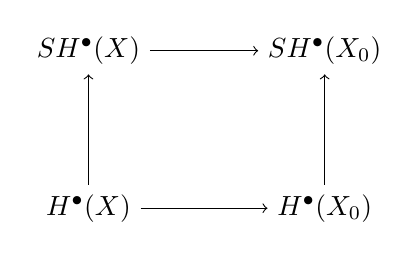
\begin{tikzpicture}

    \node (v3) at (-2,1) {$SH^\bullet(X)$};
    \node (v4) at (1,1) {$SH^\bullet(X_0)$};
    \node (v1) at (-2,-1) {$H^\bullet(X)$};
    \node (v2) at (1,-1) {$H^\bullet(X_0)$};
    \draw  (v1) edge[->] (v2);
    \draw  (v1) edge[->] (v3);
    \draw  (v3) edge[->] (v4);
    \draw  (v2) edge[->] (v4);
\end{tikzpicture}